\begin{wrapfigure}{r}{0.35\textwidth}%[h!]
\centering
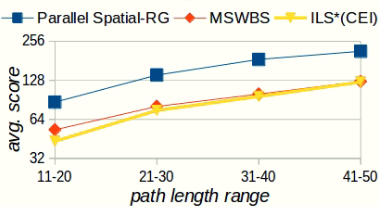
\includegraphics[width=0.35\textwidth]{candidate-london.png}
\caption{Comparison of Parallel-Spatial-RG, MSWBS, and ILS*(CEI).}
\label{fig_algo_compare}
\end{wrapfigure}
We conducted experimental analysis on the real road networks of London, Delhi, and Buenos Aires (obtained from \cite{Alireza_Karduni}). Due to lack of space, we are presenting only a summary of our results in this paper. Please refer to \cite{Venkata_M_V_Gunturi} for a detailed experimental analysis. In this paper, we present our results on the London dataset. This dataset has 285050 nodes and 749382 edges. Edges are selected uniformly at random from across the network and are assigned (randomly) a score value between 1 and 15. Other edges has 0 score value. Our experiments indicate that both the runtime and the score gain of \textit{Parallel-Spatial-RG} increases as we increase the overhead and the density of the edges with non-zero score values. Please refer to \cite{Venkata_M_V_Gunturi} for more details on this experiment. Figure \ref{fig_algo_compare} illustrates the results.